\section{Results}

% RESULTS: How successful were you at achieving your goals? We expect results sections to differ from project to project, but we expect your evaluation to be very thorough (your project evaluation is a great way to demonstrate you understood topics from this course). Here are a few ideas:
% If your project was optimizing an algorithm, please define how you measured performance. Is it wall-clock time? Speedup? An application specific rate? (e.g., moves per second, images/sec)
% Please also describe your experimental setup. What were the size of the inputs? How were requests generated?
% Provide graphs of speedup or execute time. Please precisely define the configurations being compared. Is your baseline single-threaded CPU code? It is an optimized parallel implementation for a single CPU?
% Recall the importance of problem size. Is it important to report results for different problem sizes for your project? Do different workloads exhibit different execution behavior?
% IMPORTANT: What limited your speedup? Is it a lack of parallelism? (dependencies) Communication or synchronization overhead? Data transfer (memory-bound or bus transfer bound). Poor SIMD utilization due to divergence? As you try and answer these questions, we strongly prefer that you provide data and measurements to support your conclusions. If you are merely speculating, please state this explicitly. Performing a solid analysis of your implementation is a good way to pick up credit even if your optimization efforts did not yield the performance you were hoping for.
% Deeper analysis: Can you break execution time of your algorithm into a number of distinct components. What percentage of time is spent in each region? Where is there room to improve?
% Was your choice of machine target sound? (If you chose a GPU, would a CPU have been a better choice? Or vice versa.)

\begin{figure}[h]
	\centering
	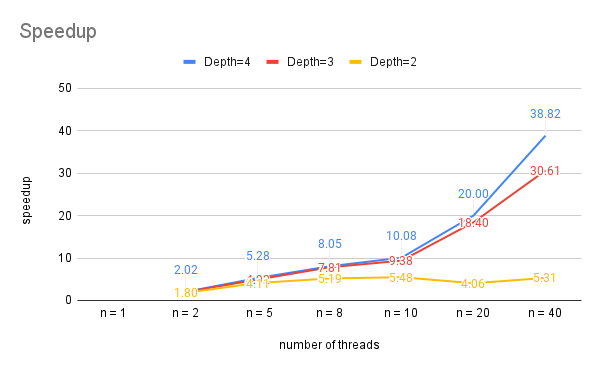
\includegraphics[width=0.45\textwidth]{speedup.png}
	\vspace{-1em}
	\caption{Approach 1 Speedup vs. Number of threads for different search depths. This figure shows that the speedup increases linearly with the number of threads.}
	\label{fig:speedup}
\end{figure}

\begin{figure}[h]
	\centering
	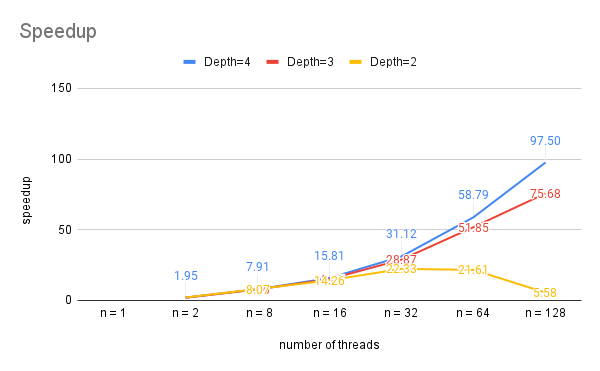
\includegraphics[width=0.45\textwidth]{Speedup_naive.png}
	\vspace{-1em}
	\caption{Approach 2 Naive Speedup vs. Number of threads for different search depths.}
	\label{fig:speedup_naive}
\end{figure}

\begin{figure}[h]
	\centering
	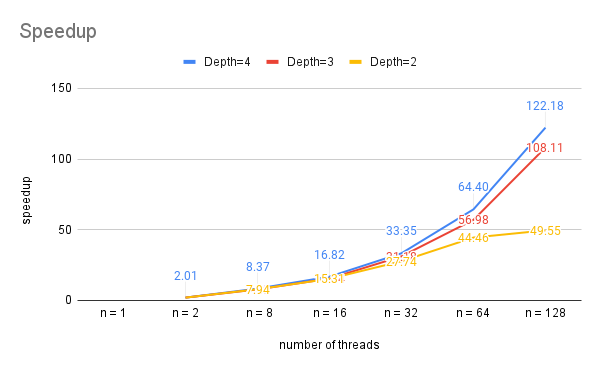
\includegraphics[width=0.45\textwidth]{Speedup_optimized.png}
	\vspace{-1em}
	\caption{Approach 2 Optimized Speedup vs. Number of threads for different search depths.}
	\label{fig:speedup_optimized}
\end{figure}

\begin{table}
\begin{tabular}{|l|r|r|r|r|r|}
\hline Depth 4 & \multicolumn{2}{|l|}{$\mathrm{n}=1$} & \multicolumn{2}{|l|}{$\mathrm{n}=128$} & ratio \\
\cline { 2 - 5 } & \multicolumn{1}{|l|}{ time(ms) } & pct(\%) & time(ms) & pct.(\%) & \\
\hline solve & $9534.483$ & $74.01 \%$ & $77.678$ & $71.29 \%$ & $1.25$ \\
\hline drop & $2451.974$ & $19.03 \%$ & $22.209$ & $20.38 \%$ & $1.61$ \\
\hline copy & $70.101$ & $0.54 \%$ & $0.591$ & $0.59 \%$ & $1.24$ \\
\hline create & 0 & $0.00 \%$ & $0.388$ & $0.36 \%$ & $5687.5$ \\
\hline other & $826.24$ & $6.41 \%$ & $8.1$ & $7.42 \%$ & $-$ \\
\hline total & $12882.80$ & $100.00 \%$ & $108.953$ & $100.00 \%$ & $1.27$ \\
\hline Depth 3 & \multicolumn{2}{|l|}{$\mathrm{n}=1$} & \multicolumn{2}{|l|}{$\mathrm{n}=128$} & ratio \\
\cline { 2 - 5 } & \multicolumn{1}{|l|}{ time(ms) } & pct(\%) & time(ms) & pct.(\%) & \\
\hline solve & $232.794$ & $77.54 \%$ & $1.892$ & $63.51 \%$ & $1.2$ \\
\hline drop & $45.863$ & $15.28 \%$ & $0.469$ & $15.74 \%$ & 2 \\
\hline copy & $1.752$ & $0.58 \%$ & $0.013$ & $0.59 \%$ & $6.36$ \\
\hline create & 0 & $0.00 \%$ & $0.396$ & $13.29 \%$ & $1045.8$ \\
\hline other & $19.81$ & $6.60 \%$ & $0.2$ & $7.02 \%$ & $-$ \\
\hline total & $300.22$ & $100.00 \%$ & $2.979$ & $100.00 \%$ & $1.68$ \\
\hline Depth 2& \multicolumn{2}{|l|}{$\mathrm{n}=1$} & \multicolumn{2}{|l|}{$\mathrm{n}=128$} & ratio \\
\cline { 2 - 5 } & \multicolumn{1}{|l|}{ time(ms) } & pct(\%) & time(ms) & pct.(\%) & \\
\hline solve & $5.803$ & $81.72 \%$ & $0.051$ & $13.32 \%$ & $94.5$ \\
\hline drop & $0.783$ & $11.03 \%$ & $0.007$ & $1.83 \%$ & $17.8$ \\
\hline copy & $0.043$ & $0.61 \%$ & $0.00034$ & $0.59 \%$ & $2.86$ \\
\hline create & 0 & $0.00 \%$ & $0.316$ & $82.51 \%$ & $395.4$ \\
\hline other & $0.47$ & $6.65 \%$ & $0.0$ & $2.26 \%$ & $-$ \\
\hline total & $7.10$ & $100.00 \%$ & $0.383$ & $100.00 \%$ & $116.5$ \\
\hline
\end{tabular}
\caption{function duration breakdown of naive approach 2.}
\label{tab:function_duration_naive}
\end{table}

\begin{table}
\begin{tabular}{|l|r|r|r|r|r|}
\hline Depth 4 & \multicolumn{2}{|l|}{$\mathrm{n}=1$} & \multicolumn{2}{|l|}{$\mathrm{n}=128$} & ratio \\
\cline { 2 - 5 } & \multicolumn{1}{|l|}{ time(ms) } & pct(\%) & time(ms) & pct.(\%) & \\
\hline solve & $8002.533$ & $79.05 \%$ & $62.937$ & $74.85 \%$ & $1.1$ \\
\hline drop & $1218.769$ & $12.04 \%$ & $12.376$ & $14.72 \%$ & $1.25$ \\
\hline copy & $70.227$ & $0.69 \%$ & $0.592$ & $0.70 \%$ & $1.48$ \\
\hline create & $0.001$ & $0.00 \%$ & $0.0002$ & $0.00 \%$ & $1.47$ \\
\hline other & $832.39$ & $8.22 \%$ & $8.2$ & $9.73 \%$ & $-$ \\
\hline total & $10123.93$ & $100.00 \%$ & $84.083$ & $100.00 \%$ & $1.09$ \\
\hline Depth 3 & \multicolumn{2}{|l|}{$\mathrm{n}=1$} & \multicolumn{2}{|l|}{$\mathrm{n}=128$} & ratio \\
\cline { 2 - 5 } & \multicolumn{1}{|l|}{ time(ms) } & pct(\%) & time(ms) & pct.(\%) & \\
\hline solve & $183.701$ & $77.63 \%$ & $1.543$ & $71.20 \%$ & $1.09$ \\
\hline drop & $31.128$ & $13.15 \%$ & $0.338$ & $15.60 \%$ & $1.4$ \\
\hline copy & $1.766$ & $0.75 \%$ & $0.014$ & $0.65 \%$ & $5.14$ \\
\hline create & $0.0001$ & $0.00 \%$ & $0.00009$ & $0.00 \%$ & $1.154$ \\
\hline other & $20.03$ & $8.47 \%$ & $0.3$ & $12.55 \%$ & $-$ \\
\hline total & $236.63$ & $100.00 \%$ & $2.167$ & $100.00 \%$ & $1.11$\\
\hline Depth 2& \multicolumn{2}{|l|}{$\mathrm{n}=1$} & \multicolumn{2}{|l|}{$\mathrm{n}=128$} & ratio \\
\cline { 2 - 5 } & \multicolumn{1}{|l|}{ time(ms) } & pct(\%) & time(ms) & pct.(\%) & \\
\hline solve & $4.578$ & $77.88 \%$ & $0.039$ & $32.50 \%$ & $75.96$ \\
\hline drop & $0.778$ & $13.24 \%$ & $0.009$ & $7.50 \%$ & $38.58$ \\
\hline copy & $0.043$ & $0.73 \%$ & $0.0003$ & $0.25 \%$ & $2.86$ \\
\hline create & $0.00006$ & $0.00 \%$ & $0.0001$ & $0.08 \%$ & $1.09$ \\
\hline other & $0.48$ & $8.15 \%$ & $0.1$ & $59.67 \%$ & $-$ \\
\hline total & $5.88$ & $100.00 \%$ & $0.12$ & $100.00 \%$ & $1.12$\\
\hline
\end{tabular}
\caption{function duration breakdown of optimized approach 2.}
\label{tab:function_duration_optimized}
\end{table}
In this section, we present the results for the experiments we conducted on the GHC and PSC machines. We focused our experiments on approach2 since it has the best performance and also the most flexible design. 

\subsection{Approach 1 Naive DFS}
Our first experiment measures the speedup with different number of threads for the approach 1 parallelized OpenMP DFS search algorithm for different search depths. A graph of the experiment is shown in Fig. \ref{fig:speedup}. Here we only show the speedup up to 40 threads since the DFS algorithm can't support threads more than 40. We can observe from the graph that as the search depth increases, the speedup approaches linear speedup to the number of threads used. We think the reason is that shallower depth results in smaller search space and the overhead of searching for the optimal position and orientation outweighs the speedup benefits. However, later we discover that the main reason for the sub-optimal speedup is because of a lock shared between the threads which we would discuss in later sections. Since this approach limited the number of thread we can use, we didn't further optimize this approach.

\subsection{Approach 2 Before Optmization}
The next experiment measures the speedup with different number of threads for the Approach 2 parallelized method for different search depths. The graph of this experiment is shown in Fig. \ref{fig:speedup_naive}. This experiment is conducted on n=1 to n=128 threads. We can observe the same trend of speedup approaching linear to the number of threads used as the search depth increases. However, the speedup is not perfect for n = 64 and n = 128. This is due to the workload imbalance we mentioned in the previous section. As for depth = 2, we observed the same performance downgrade in the Approach 1 for high number of threads. 

To further investigate the non-linear speedup for shallower search depths, we conduct our third experiment, which measures the duration of each function. The results of this experiment is displayed in Table. \ref{tab:function_duration_naive}. For this experiment, we measure the execution time of four main functions that is necessary during our DFS search for different search depths using 1 and 128 threads, respectively. We used C function gettimeofday which has the granularity of microseconds. The overhead of the time measurement is under 1us so wouldn't affect the solver performance. 
In the table, we measure 4 crucial function including solve, drop, copy and create. The solve function denotes the tg\_get\_score() function, which is used to calculate the score of a game state. The drop function denotes the tg\_drop() function, which drops the falling block into place after the block position (column) has been determined. The copy function denotes the tg\_copy() function, which copies the tetris game solver, this is needed because we want to resume the board state. The create function denotes the tg\_create() function, which creates a new tetris game solver function. We measured tg\_create() because we discovered it was the bottleneck for shallower depth, especially for depth = 2. 
Additionally, we also measure the maximum and minimum execution time of each function between different threads and define ratio as maximum / minimum, the larger ratio is, the more imbalance the function workload is.  

We can observe from Table. \ref{tab:function_duration_naive} for depth 3 and 4, most execution time is on solve and drop accounting for over 85\% of the work time, which is what we expected. However, there is a slight workload imbalance of the two function (1.2 and 1.6 for depth = 4) that limits our speedup from reaching perfect speedup. The overhead of multiple threads here are still small with around 7\% of total time. As for depth = 2, we can see that the execution time is mostly on tg\_create() which is abnormal. The ratio of tg\_create() in all depth is also unreasonably large. After some dig in, we find that it was because the same problem we encounter earlier, there was a srand() function call in tg\_create() that acquires a lock betweens threads. Therefore, we removed this srand() in the optimized version of approach 2. 

\subsection{Approach 2 After Optimization}
Here we present the result of our optimized approach 2, we applied the three optimization mentioned in optimization section and also fixed the srand() locking problem. The speedup result is shown in Fig. \ref{fig:speedup_optimized}. We can see that depth = 4 reached near perfect speedup (122.18) after we optimized the workload imbalance of the tg\_get\_score() function. As the depth decrease, the overheads takes in effect and the speedup is lowered, as depth = 2 has only 49.55 speedup, however this is still much higher than the naive version (5.41). 

From Table. \ref{tab:function_duration_optimized} there is 4 things worth pointing out. First, the tg\_create() is no longer a bottleneck for depth = 2 n = 128, instead other are now the main reason for the performance slowdown. This is expected since we fixed the lock problem. Second, as the depth decrease, the other percentage also increase, especially in depth = 2, where 60\% of the time is on other. This is expected since other represents the overhead and the overhead increase as depth decrease since we have less calculation for each thread. Third, the drop function time for depth = 4 decreased from 20\% to 15\%, indicating our caching is effective. Finally, we can see that nearly all ratio decrease for all depth, which implies that our optimization has successfully solve the workload imbalance, resulting in better speedup. 